\chapter[Planificación y costes]{
  \label{chp:planificacion}
  PLANIFICACIÓN Y COSTES
}
\thispagestyle{numberingStyle}
\pagestyle{numberingStyle}



\section{Planificación}

\subsection{División de las tareas}
Para las iteraciones definidas anteriormente se establecerá una división en tareas, sobre las que se realizará la planificación necesaria para obtener la estimación del esfuerzo requerido en cada iteración.

A continuación, se mostrará las diferentes tareas que componen cada una de las iteraciones junto con los valores del tiempo necesario para su realización (en horas).

\subsubsection*{Iteración 1: Análisis de requisitos y diseño}

\begin{figure}[H]
\vspace{-0.5cm}
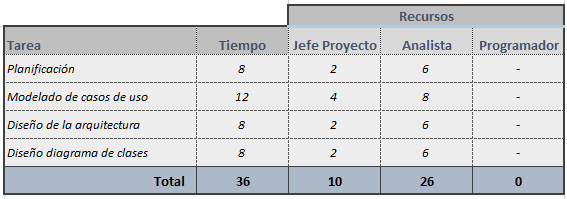
\includegraphics[
   keepaspectratio=true
]{./03_Met_Plan/02_Planificacion/img/PlanIter1.png}
\caption{Diagrama división tareas - iteración 1}
\end{figure}


\subsubsection*{Iteración 2: Base inicial proyecto}

\begin{figure}[H]
\vspace{-1cm}
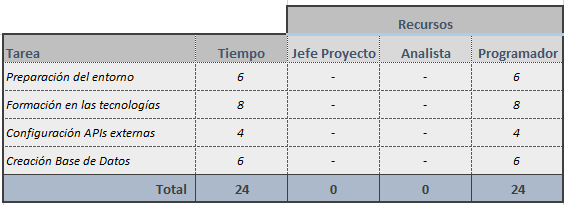
\includegraphics[
   keepaspectratio=true
]{./03_Met_Plan/02_Planificacion/img/PlanIter2.png}
\caption{Diagrama división tareas - iteración 2}
\end{figure}


\subsubsection*{Iteración 3: Usuarios}

\begin{figure}[H]
\vspace{-1cm}
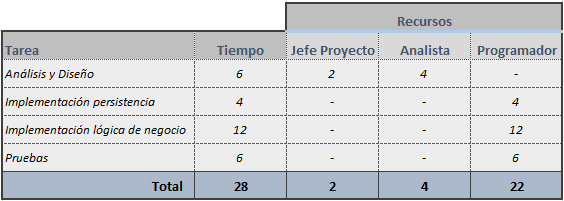
\includegraphics[
   keepaspectratio=true
]{./03_Met_Plan/02_Planificacion/img/PlanIter3.png}
\caption{Diagrama división tareas - iteración 3}
\end{figure}


\subsubsection*{Iteración 4: Rutas}

\begin{figure}[H]
\vspace{-1cm}
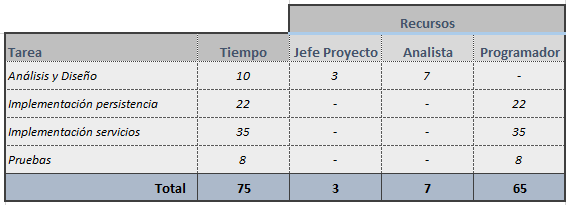
\includegraphics[
   keepaspectratio=true
]{./03_Met_Plan/02_Planificacion/img/PlanIter4.png}
\caption{Diagrama tareas iteración 4}
\end{figure}



\subsubsection*{Iteración 5: Eventos}

\begin{figure}[H]
\vspace{-1cm}
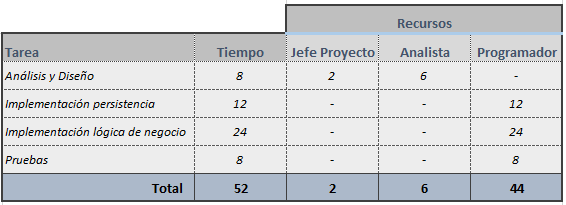
\includegraphics[
   keepaspectratio=true
]{./03_Met_Plan/02_Planificacion/img/PlanIter5.png}
\caption{Diagrama división tareas - iteración 5}
\end{figure}


\subsubsection*{Iteración 6: Servicios externos}

\begin{figure}[H]
\vspace{-1cm}
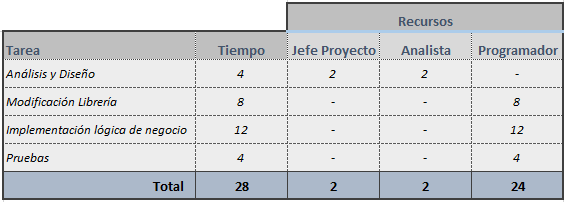
\includegraphics[
   keepaspectratio=true
]{./03_Met_Plan/02_Planificacion/img/PlanIter6.png}
\caption{Diagrama división tareas - iteración 6}
\end{figure}


\subsubsection*{Iteración 7: Lugares y categorías}

\begin{figure}[H]
\vspace{-1cm}
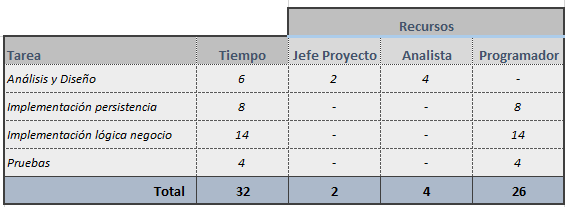
\includegraphics[
   keepaspectratio=true
]{./03_Met_Plan/02_Planificacion/img/PlanIter7.png}
\caption{Diagrama tareas iteración 7}
\end{figure}


\subsubsection*{Iteración 8: Capa servicios}

\begin{figure}[H]
\vspace{-1cm}
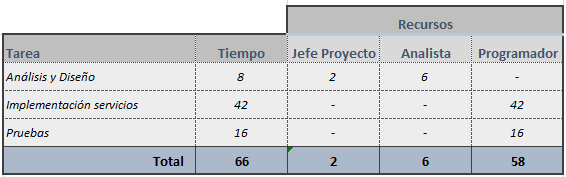
\includegraphics[
   keepaspectratio=true
]{./03_Met_Plan/02_Planificacion/img/PlanIter8.png}
\caption{Diagrama división tareas - iteración 8}
\end{figure}


\subsubsection*{Iteración 9: Autenticación y autorización}

\begin{figure}[H]
\vspace{-1cm}
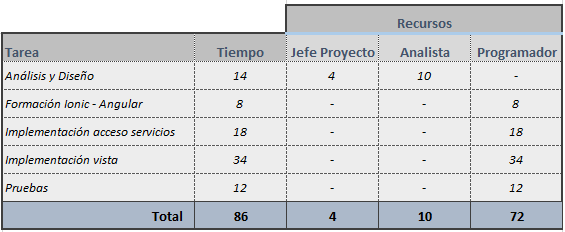
\includegraphics[
   keepaspectratio=true
]{./03_Met_Plan/02_Planificacion/img/PlanIter9.png}
\caption{Diagrama división tareas - iteración 9}
\end{figure}


\subsubsection*{Iteración 10: Cliente móvil}

\begin{figure}[H]
\vspace{-1cm}
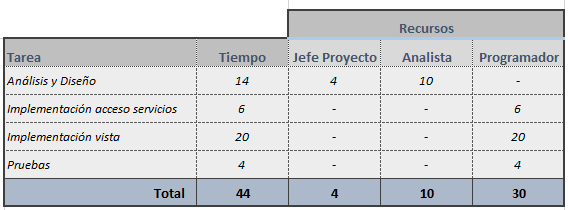
\includegraphics[
   keepaspectratio=true
]{./03_Met_Plan/02_Planificacion/img/PlanIter10.png}
\caption{Diagrama división tareas - iteración 10}
\end{figure}


\subsubsection*{Iteración 11: Cliente web}

\begin{figure}[H]
\vspace{-1cm}
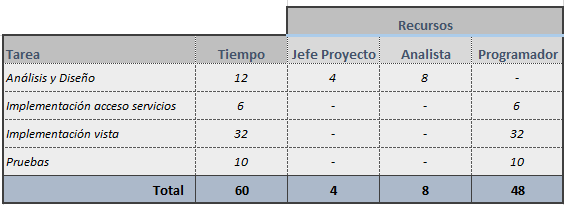
\includegraphics[
   keepaspectratio=true
]{./03_Met_Plan/02_Planificacion/img/PlanIter11.png}
\caption{Diagrama división tareas - iteración 11}
\end{figure}


\subsubsection*{Iteración 12: Panel de administración}

\begin{figure}[H]
\vspace{-1cm}
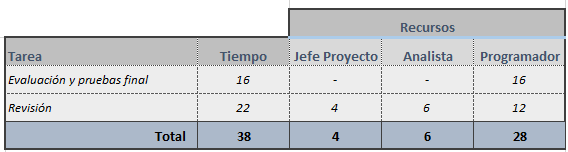
\includegraphics[
   keepaspectratio=true
]{./03_Met_Plan/02_Planificacion/img/PlanIter12.png}
\caption{Diagrama división tareas - iteración 12}
\end{figure}


\subsubsection*{Iteración 13: Cierre}

\begin{figure}[H]
\vspace{-1cm}
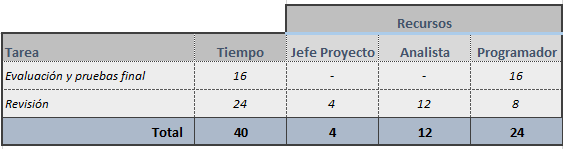
\includegraphics[
   keepaspectratio=true
]{./03_Met_Plan/02_Planificacion/img/PlanIter13.png}
\caption{Diagrama división tareas - iteración 13}
\end{figure}


\subsubsection*{Planificación global}

\begin{figure}[H]
\vspace{-0.5cm}
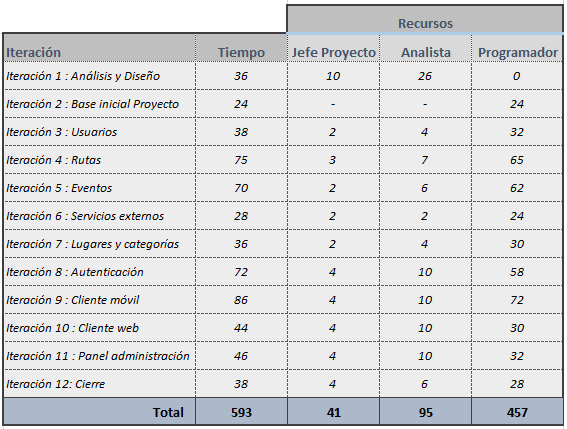
\includegraphics[
   keepaspectratio=true
]{./03_Met_Plan/02_Planificacion/img/PlanIterGlobal.png}
\caption{Diagrama división tareas - global}
\end{figure}

\newpage
\subsection{Planificación de las tareas}
En el siguiente diagrama se podrá observar la planificación total de proyecto así como la establecida en cada iteración.

\begin{figure}[H]
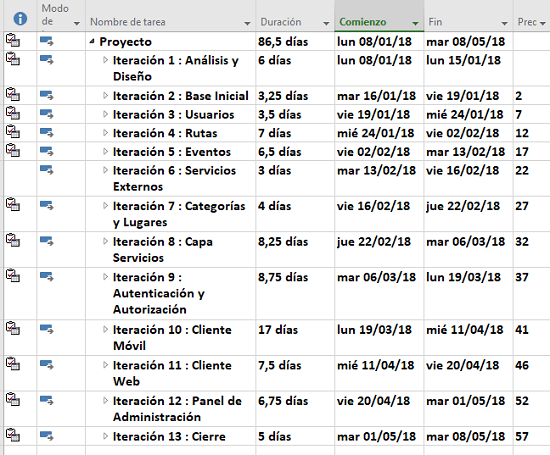
\includegraphics[
   keepaspectratio=true
]{./03_Met_Plan/02_Planificacion/img/gantt1.png}
\caption{Diagrama planificación - global}
\end{figure}

Observando el diagrama se puede observar la duración, la fecha de comienzo y de fin para el proyecto entero. Se muestra también la división y planificación del mismo, en las diferentes iteraciones definidas previamente. Para cada iteración, también se puede observar la planificación realizada.

En los siguiente diagramas se mostrará la planificación de las tareas para cada una de las iteraciones, indicando para cada una de ellas, el nombre, la fecha de inicio y fin, la duración, las tareas predecesoras y los recursos asignados encargados de realizar dicha tarea.


\begin{sidewaysfigure}
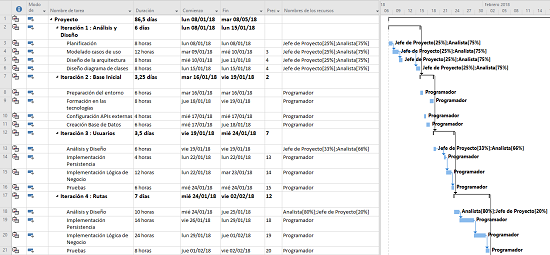
\includegraphics[
   keepaspectratio=true
]{./03_Met_Plan/02_Planificacion/img/gantt2.png}
\caption{Diagrama planificación - iteraciones 1-4}
\end{sidewaysfigure}

\begin{sidewaysfigure}
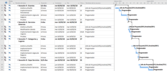
\includegraphics[
   keepaspectratio=true
]{./03_Met_Plan/02_Planificacion/img/gantt3.png}
\caption{Diagrama Gantt - iteraciones 5-8}
\end{sidewaysfigure}

\begin{sidewaysfigure}
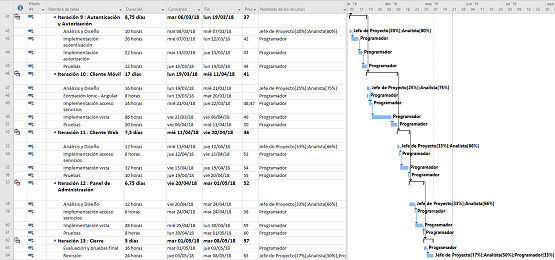
\includegraphics[
   keepaspectratio=true
]{./03_Met_Plan/02_Planificacion/img/gantt4.png}
\caption{Diagrama Gantt - iteraciones 9-13}
\end{sidewaysfigure}




\section{Evaluación de costes}
\subsection{Recursos Humanos}
En la planificación del proyecto se han distinguido diferentes perfiles profesionales involucrados en la realización de las diferentes tareas. Conociendo el número total de horas trabajadas por cada recurso y su coste por hora, podemos calcular el coste total, de todos los recursos humanos, en el proyecto.

\begin{table}[H]
\centering
\begin{tabular}{|l|c|c|c|}
\hline
\textbf{Recurso} & \textbf{Coste/hora} & \textbf{Horas Trabajadas} & \textbf{Coste Total} \\ \hline
Jefe de Proyecto & 20 €/h & 38 & 760 €  \\ \hline
Analista & 18 €/h & 92 &  1.656 €  \\ \hline
Programador & 16 €/h & 492 & 7.872 €  \\ \hline
\textbf{Total} & & & \textbf{10.288 €} \\ \hline
\end{tabular}
\caption{Coste recursos humanos}
\end{table}


\subsection{Costes Hardware}
En cuanto al coste hardware se contabilizará únicamente los equipos utilizados para el desarrollo del proyecto. Una vez que la aplicación se lleve a la etapa de producción, se deberán contabilizar los gastos que supondrían mantener los servidores y equipos necesarios para su correcto funcionamiento.

En el desarrollo se ha empleado un ordenador personal del autor, con un coste aproximado de 1.300 euros.


\subsection{Costes Software}
Las principales herramientas software utilizadas en el desarrollo del proyecto son gratuitas. Únicamente, destacar el uso de una versión para estudiantes gratuita del software MagicDraw, y el uso de las versiones estándar de las APIs de Foursquare y Google que implican una serie de límites y restricciones, asumibles en el desarrollo y pruebas de la aplicación. 

Al igual que sucedía con los costes hardware, cuando la aplicación se encuentre en producción, será necesario asumir el coste de las versiones premium de las APIs mencionadas.


\subsection{Costes totales}
Como resultado de cada uno de las estimaciones de costes correspondientes a los recursos humanos, hardware y software; podemos estimar el coste total del desarrollo del proyecto.

\begin{table}[H]
\centering
\begin{tabular}{|l|c|c|c|}
\hline
\textbf{Recurso} & \textbf{Coste Total} \\ \hline
Recursos Humanos &  10.288 € \\ \hline
Hardware & 1.300 €  \\ \hline
Software & 0 €  \\ \hline
\textbf{Total} & \textbf{11.588 €} \\ \hline
\end{tabular}
\caption{Coste recursos humanos}
\end{table}

Finalmente, se obtiene un coste total de 11.588 €.
